\documentclass[9pt]{beamer}
%\usetheme{Malmoe}
\usetheme{Darmstadt}
\usecolortheme{beaver}
\setbeamertemplate{navigation symbols}{}
\beamersetuncovermixins{\opaqueness<1>{25}}{\opaqueness<2->{15}}
\usepackage{url}
\usepackage{ragged2e}
\usepackage{multirow}
\usepackage{minted}
%\usepackage{color}
\usepackage{subfigure}
%\usepackage[square,sort&compress]{natbib} 
\usepackage{graphics}
\usepackage{epsfig}
\usepackage{times}
\usepackage{amsmath}
\usepackage{amssymb}
\usepackage{color}
\usepackage{algorithm}
\usepackage{algorithmic}
\usepackage{multirow}
\def\imagetop#1{\vtop{\null\hbox{#1}}}

\definecolor{blue}{rgb}{.1,.1,.5}
\definecolor{lightblue}{rgb}{.1,.1,.9}
\definecolor{darkred}{rgb}{.7,.1,.1}
\definecolor{bg}{rgb}{.9,.9,.1}
\def\slantfrac#1#2{\kern.1em^{#1}\kern-.3em/\kern-.1em_{#2}}

\logo{
\includegraphics[width=1in]{pics/UdeM_NoirBleu_logo_Marie_crop.pdf}}
% Standard LaTeX stuff - note the optional abbreviated title being provided
\title[Description of ift6266h12 repo]{Description of ift6266h12 repo}
\author[Razvan Pascanu]{Razvan Pascanu\\ Professeur: Yoshua Bengio}

\date{\today}

\setbeamertemplate{footline}{\hspace*{.5cm}\scriptsize{Razvan Pascanu  ---
Description of ift6266-h12 repository
\hspace*{50pt} \hfill\insertframenumber\hspace*{.5cm}}} 
\renewcommand{\theFancyVerbLine}{\sffamily
\textcolor[rgb]{0.5,0.5,1.0}{\scriptsize
\oldstylenums{\arabic{FancyVerbLine}}}}

\begin{document}


\frame{\titlepage}


\section{Grabbing the repository}
\subsection{Git and Assembla}
\begin{frame}
    %\frametitle{Git and Assmebl a}
        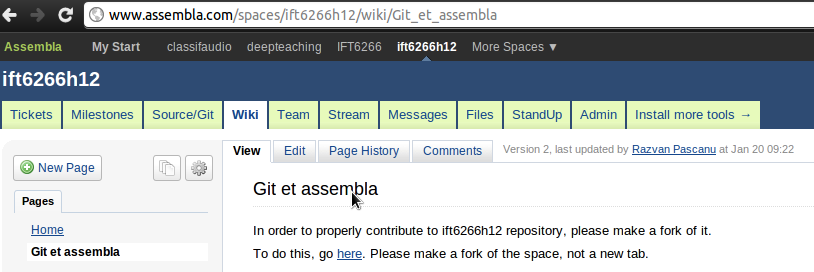
\includegraphics[width=.8\textwidth]{pics/assembla.png} 
    \begin{itemize}
        \item Repo: \url{http://www.assembla.com/spaces/ift6266h12/wiki}
    \end{itemize}
    {\color{darkred}TODO}:
    \begin{itemize}
        \item Make sure to have your public key registered with assembla
        \item Create a fork of the repository
        \item Learn to properly use {\color{darkred} Git}
    \end{itemize}
\end{frame}

\subsection{Clone the repository}
\begin{frame}[fragile]

    \definecolor{bg}{rgb}{.9,.9,.9}
    \begin{minted}[linenos=True, bgcolor=bg, frame=lines]{sh}
echo $PYTHONPATH
cd $HOME/repos
git clone git@git.assembla.com:user-ift6266h12-fork.git
ln -s user-ift6266h12/ift6266h12 ift6266h12
cd user-ift6266h12
git remote add central \
    git@git.assembla.com:ift6266h12.git
git fetch central
git checkout -b pca_terry central/master
...
git add -p
git commit
git push origin pca_terry
    \end{minted}
    \begin{itemize}
      \item  http://deeplearning.net/software/theano/dev\_start\_guide.html
    \end{itemize}
\end{frame}

\section{Repository Structure}
\begin{frame}
 \begin{itemize}
    \item \emph{utils} folder containing I/O functionaly
        \begin{itemize}
            \item load\_train\_input
            \item load\_train\_labels
            \item load\_valid\_input
            \item load\_test\_input
        \end{itemize}
    \item \emph{server} folder containing code simulating the UTLC server
 \end{itemize}
 \end{frame}

\begin{frame}[fragile]
 \begin{itemize}
    \item Data is stored in 
    \begin{minted}{sh}
    /data/lisa/data/UTLC
    \end{minted}
 \end{itemize}
    
    \definecolor{bg}{rgb}{.9,.9,.9}
    \begin{minted}[linenos=True, bgcolor=bg, frame=lines]{sh}
if [ -e "/opt/lisa/os/.local.bashrc" ];\
    then source /opt/lisa/os/.local.bashrc;\
    else source /data/lisa/data/local_export/.local.bashrc;\
fi
    \end{minted}
\end{frame}

\section{SciKits}
\begin{frame}
 \begin{itemize}
    \item Python library for machine learning (numpy/scipy based)
    \item well docummented 
    \item stable
    \item diverse
    \item pure-python implementation !
    \item offers \emph{PCA} and \emph{RandomizedPCA}
    \item \url{http://scikit-learn.org/stable/}
 \end{itemize}
\end{frame}

\section{Pylearn2}
\begin{frame}
    \begin{itemize}
  \item ML-library developed in the LISA lab (we had a pylearn and plearn before)
  \item based on Theano
  \item tries to be flexible yet simple to draft known algorithms
  \item not that well documented
  \item not ready for prime time
    \end{itemize}
\end{frame}

\begin{frame}
    \begin{itemize}
        \item GO through the code for running a De-noising AutoEncoder
        \item GO to the PCA implementation
    \end{itemize}
\end{frame}

\begin{frame}
    \begin{itemize}
    \item Offers implementation for PCA
    \item I got confusing signals regarding the quality of the code
    \item It seems last year people mostly relied on scikits
    \end{itemize}
\end{frame}
\section{Questions}
\begin{frame}
    \begin{center}
    {\Huge Questions ? }
    \end{center}
\end{frame}
\end{document}
